\documentclass{article}

%package setup
\usepackage{graphicx}
\usepackage{amsmath}
\usepackage{fancyhdr}
\usepackage[margin=1in]{geometry}
\usepackage{comment}
\usepackage{placeins}
\usepackage{parskip}
\usepackage{subcaption}
\usepackage{appendix}
\usepackage{soul}
\usepackage{comment}
\PassOptionsToPackage{hyphens}{url}\usepackage[hidelinks]{hyperref}
\usepackage{matlab-prettifier}
\usepackage{minted}
\usepackage{enumitem}
\usepackage{float}
\usepackage{textcomp, gensymb}
\usepackage{caption}


\pagestyle{fancy}
\fancyhf{} % Clear header/footer settings
\rhead{\thepage} % Page number on the right in the header
\lhead{ASE375 Lab Report 8} % Your lab report title on the left

\begin{document}

\begin{titlepage}
  \centering
  
\includegraphics[width=10cm]{ase-logo-formal.png}  % Adjust the width as needed
  \vspace{1cm}  % Add some vertical space
 
  \Large \textbf{ASE 375 Electromechanical Systems}\\
  \large \textbf{Section 14115}\\
  \vspace{0.5cm}
  \textbf{Monday: 3:00 - 6:00 pm}\\
 
  \vspace{1cm}
 
  \hrule
  \vspace{0.5cm}
 
  \Huge \textbf{Report 8:\\
    Landing Gear Drop Test}\\
  \Huge \textbf{}\\
 
  \vspace{0.5cm}
  \hrule
 
  \vspace{1cm}
 
  \normalsize \textbf{Andrew Doty, Andres Suniaga, Dennis Hom}\\
  \normalsize \textbf{Due Date: 04/08/2024}
 
\end{titlepage}
\newpage

\tableofcontents
\thispagestyle{empty}
\newpage

\section{Introduction}
In this experiment we take a look at the transient response of a landing gear as it is dropped from various heights. Drop tests are a useful measure to verify the performance and safety of an aircraft. In this lab we use a small scale landing gear equipped with a rotary potentiometer to measure the angle of the landing gear linkage and a piezoelectric accelerometer to measure the acceleration of it's response. From the potentiometer data we can calulate the stroke of the landing gear, which represents the compression or stretching of the spring attached to the landing leg.
\vspace{2.5mm}

Using a laser pointer and a photo-diode, we are able to perform triggered data acquisition of the transient response of the landing gear as it makes impact with the table surface. These triggered measurements allow us to gather consistent and time-resolved data for each drop height.

\section{Equipment}
Measurement devices and hardware used in this lab include:
\begin{itemize}

\item Small-Scale Landing Gear: 
\vspace{1mm}

Scaled-down landing gear used for drop testing. Setup shown in Figure \ref{fig:gearsetup}

\begin{figure}[H]
    \centering
    \frame{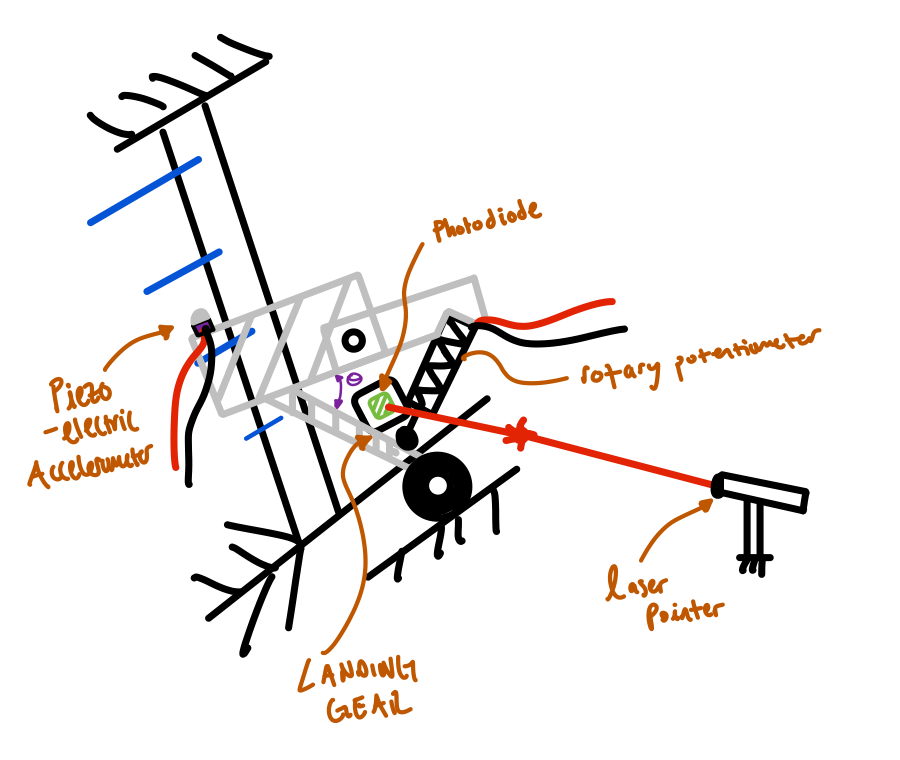
\includegraphics[width=0.65\textwidth]{lab8images/landinggearsetuplab8.png}}
    \caption{Landing Gear Drop Test Setup}
    \label{fig:gearsetup}
\end{figure}

\vspace{2.5mm}

\item Piezoelectric Accelerometer \hyperlink{2}{[2]}:
\vspace{1mm}

The Piezoelectric accelerometer only measures acceleration in one direction, and is placed on the small-scale landing gear as shown in Figure \ref{fig:gearsetup}.\\[1mm]
The operational principle of the Piezoelectric accelerometer is in it piezoelectric crystal, which generates charge from applied stress. It converts mechanical energy into electrical energy. The crystal acts like a capacitor (stores electrical energy). Operational Voltage = $5\text{V}$
\vspace{2.5mm}

\item Laser Pointer (Red, $\gamma \approx 700\; \text{nm}$) and Silicon Photodiode \hyperlink{3}{[3]}:
\vspace{1mm}

For this setup, a red laser pointer shines on the Si photodiode until interrupted by the dropped landing gear at which a response is triggered and we are able to model this transient response of the landing gears impact.\\[1pt]
The Si photodiode is able to convert optical power into electrical current, which as seen in Figure \ref{fig:diodecircuit}, allow passage of current when the diode is triggered or interrupted by the landing gear, allowing us to get the time-resolved $V_{OUT}$ measurements for each height drop.
\vspace{2.5mm}

\item Rotary Potentiometer:
\vspace{1mm}

The rotary potentiometer is used to calculate the angle $\theta$ between the landing gear leg and the structure it is fixed on as seen in Figure \ref{fig:gearsetup}.\\[1pt] The working principle of the rotary potentiometer is angular movement. There is a shaft or knob which varies resistance as it is turned.

\vspace{2.5mm}

\item DAQ, NI-9215 Voltage Input Module \hyperlink{datasheets}{[1]},  and LabVIEW:
\vspace{1mm}

Data Acquisition System used to process sample measurements into digital data for the computer to read.\\[5pt]
NI-9215 is an analog input module used to measure the output voltage signals of the sensors.\\[5pt]
LabVIEW used to model these output voltages read from the DAQ of the piezo-electric accelerometer, photodiode, and rotary potentiometer.

\item Solderless Breadboard, Jumper Wires, $1\; \text{k}\Omega$ Resistor, $0.1\; \micro\text{F}$ Capacitor, and $10\; \text{k}\Omega$ Resistor: 
\vspace{1mm}

Used to make connections to the input analog modules and to construct circuits. In this lab, we construct a circuit as shown in Figure \ref{fig:diodecircuit} with the $1\; \text{k}\Omega$ Resistor and  $0.1\; \micro\text{F}$ Capacitor serving as the noise filter. The $10\; \text{k}\Omega$ Resistor is reached only if the laser to the diode is interrupted by the landing gear, which will trigger the measurements to begin.

\begin{figure}[H]
    \centering
    \frame{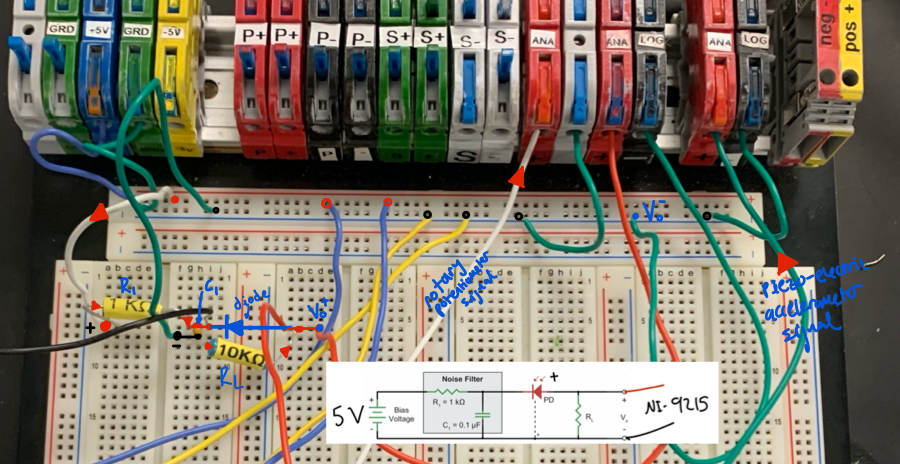
\includegraphics[width=\textwidth]{lab8images/circuitlab8_.png}}
    \caption{Photodiode Circuit on Breadboard}
    \label{fig:diodecircuit}
\end{figure}

\end{itemize}

\section{Procedure}
Before beginning the experiment, setup the LabVIEW model to output the data from the photo-diode, potentiometer, and piezoelectric accelerometer:

\begin{figure}[H]
    \centering
    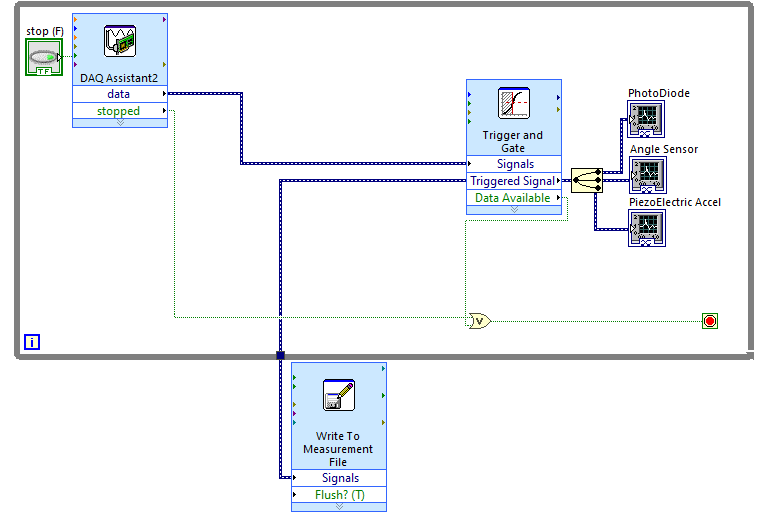
\includegraphics[width=0.65\textwidth]{lab8images/lab8blockdiag.PNG}
    \caption{LabVIEW Experiment Setup}
    \label{fig:labview}
\end{figure}

Run this model and test a few landing gear drops to ensure there is (correct) output measurements. 

\subsection{Drop Testing}
\begin{enumerate}
    \item Turn on the laser pointer so that it is shining directly onto the photodiode.
    \item Mark 3-5 different heights to drop the landing gear from. Measured from the surface at which the wheel rests, we chose to drop the landing gear at these heights in centimeters:
    \begin{center}
            \(\textbf{h} = \left[18,\, 36,\, 54,\, 72\right]\)
    \end{center}
    \item For each $h_{i}$, raise the landing gear such that the bottom of the wheel sits atop the measurement marker. Start the LabVIEW model and then drop the landing gear. This should interrupt the photodiode as it passes through the laser pointers ray and trigger a response on the LabVIEW plots. This will be the transient response. Save each of the sensors measurements to a file.
    \item After performing the landing gear drop test at each height, move on to \hyperlink{datapro}{Data Processing} to plot this transient acceleration and landing gear stroke for each $h_{i}$.
    \end{enumerate}

\hypertarget{datapro}{}
\section{Data Processing}
\subsection{Variables and Equations}  

Calibrated Output Voltage:
\begin{equation}
    V_{OUT_c} = |V_{OUT} - V_{o}|
\end{equation}

Variables:
\begin{itemize}
    \item \(V_{OUT}\): Output Voltage measurement from DAQ
    \item \(V_{o}\): Initial voltage prior to drop
\end{itemize}
\vspace{5mm}

Piezo-electric Measured Transient Accleration:
\begin{equation}
    \ddot{x} = \dfrac{V_{OUT_c}}{C_{\text{piezo}}}
\end{equation}

Variables:
\begin{itemize}
    \item \(C_{\text{piezo}} = 10\; \text{mV/g}\): Piezo-electric Accelerometer Calibration Constant
\end{itemize}
\vspace{5mm}

Law of Cosines:
\begin{equation}
    c = \sqrt{a^{2} + b^{2} - 2ab\cos{(\theta)}}
\end{equation}

Variables:
\begin{itemize}
    \item \(a,\, b\): Lengths in inches of the landing gear leg
\end{itemize}

\begin{figure}[H]
    \centering
    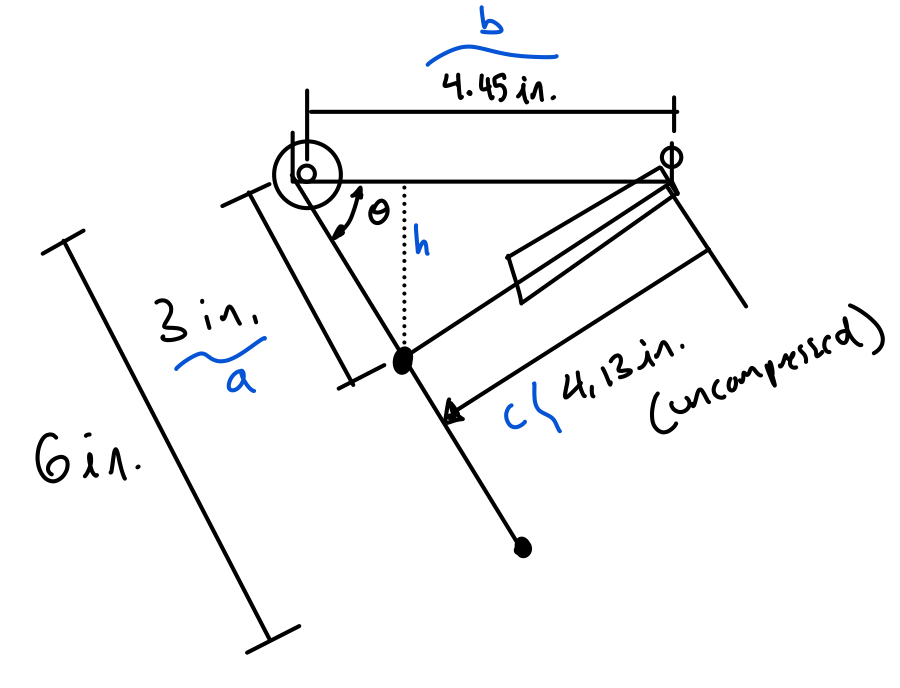
\includegraphics[width = 0.45\textwidth]{lab8images/landinggeardimensions.png}
    \caption{Dimensions of the Small-Scale Landing Gear}
    \label{fig:geardimensions}
\end{figure}
\vspace{5mm}

Area of a Triangle (Heron's Formula):
\begin{equation}
    A = \sqrt{s(s-a)(s-b)(s-c)}
\end{equation}

Variables:
\begin{itemize}
    \item \(s = \dfrac{a+b+c}{2}\): Semi-perimeter
\end{itemize}
\vspace{5mm}

Height of a Triangle:
\begin{equation}
    h = \dfrac{2A}{b}
\end{equation}

Stroke Length:
\begin{equation}
    y = h_{o} - h
\end{equation}

Variables:
\begin{itemize}
    \item \(h_{o}\): Uncompressed height, Figure \ref{fig:geardimensions}. 
\end{itemize}
\vspace{5mm}
\section{Results and Analysis}

 
\section{Conclusion}



\newpage
\thispagestyle{empty}  % Clear header/footer
\begin{center}
	\vspace*{\fill}
	{\Huge Appendix}
	\vspace*{\fill}
\end{center}

% Start appendices
\newpage
\begin{appendices}
\pagestyle{fancy}
\renewcommand{\thefigure}{A\arabic{figure}}
\setcounter{figure}{0}

% \section*{t-Distribution Tables}
% \hypertarget{1}{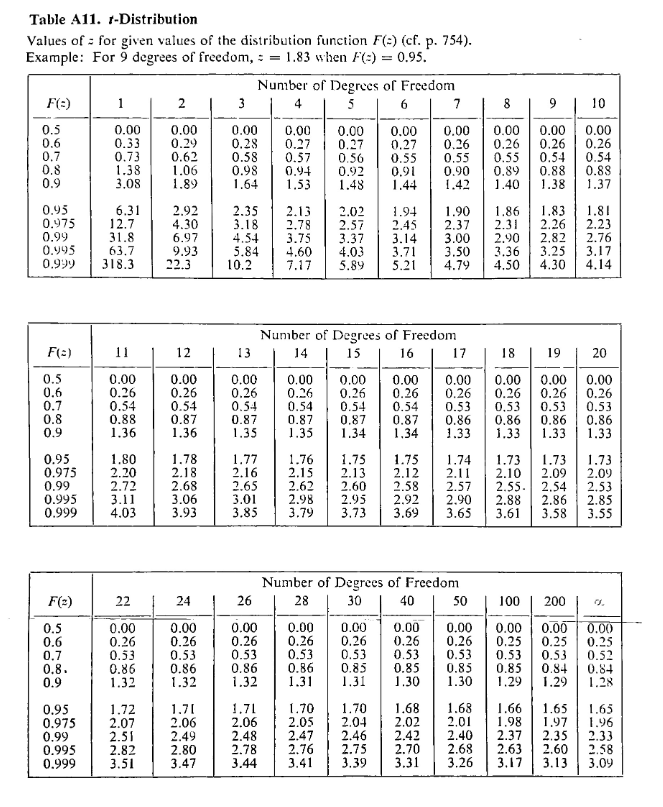
\includegraphics[width=0.95\textwidth]{t_distribution_Table_lecture3.png}}

%Add other appendix items here

\pagebreak

\hypertarget{datasheets}{}
\section{Datasheets}
\begin{enumerate}[label = {[\arabic*]}]
\small
\item \textbf{NI-9215 Datasheet:}\\[2pt] \url{https://www.amc-systeme.de/files/pdf/ni-9215-amc.pdf}
\item \hypertarget{2}{\textbf{Piezo-electric IMI Series 660 Accelerometer:}}\\[2pt] \url{https://pim-kft.hu/wp-content/uploads/2016/02/PCB_LowCost_Embeddable_Accelerometers.pdf}
\item \hypertarget{3}{\textbf{Silicon Photodiode, FDS1010:}}\\[2pt] \url{https://www.thorlabs.com/drawings/e7e91d1f442ec5dc-834C7101-FD1F-1B62-609D921F0FC0E314/FDS1010-SpecSheet.pdf}
\item \hypertarget{4}{\textbf{QP-2H Rotary Potentiometer}}\\[2pt] \url{https://www.diltronic.com/wp-content/uploads/2020/03/DILTRONIC-QP-2H-serie-datasheet.pdf}


\end{enumerate}

\end{appendices}

\end{document}
